%%%%%%%%%%%%%%%%%%%%%%%%%%%%%%%%%%%%%%%%%
% baposter Landscape Poster
% LaTeX Template
% Version 1.0 (11/06/13)
%
% baposter Class Created by:
% Brian Amberg (baposter@brian-amberg.de)
%
% This template has been downloaded from:
% http://www.LaTeXTemplates.com
%
% License:
% CC BY-NC-SA 3.0 (http://creativecommons.org/licenses/by-nc-sa/3.0/)
%
%%%%%%%%%%%%%%%%%%%%%%%%%%%%%%%%%%%%%%%%%

%----------------------------------------------------------------------------------------
%	PACKAGES AND OTHER DOCUMENT CONFIGURATIONS
%----------------------------------------------------------------------------------------

\documentclass[portrait,a0paper,fontscale=0.285]{baposter} % Adjust the font scale/size here

\usepackage{graphicx} % Required for including images
\usepackage[normalem]{ulem}
\usepackage{macros}

\usepackage{amsmath} % For typesetting math
\usepackage{amssymb} % Adds new symbols to be used in math mode

\usepackage{booktabs} % Top and bottom rules for tables
\usepackage{enumitem} % Used to reduce itemize/enumerate spacing
\usepackage{palatino} % Use the Palatino font
\usepackage[font=small,labelfont=bf]{caption} % Required for specifying captions to tables and figures

\usepackage{multicol} % Required for multiple columns
\setlength{\columnsep}{1.5em} % Slightly increase the space between columns
\setlength{\columnseprule}{0mm} % No horizontal rule between columns

\usepackage{tikz} % Required for flow chart
\usetikzlibrary{shapes,arrows} % Tikz libraries required for the flow chart in the template

%\usepackage[round]{natbib}   % omit 'round' option if you prefer square brackets
%\bibliographystyle{plainnat}

\begin{document}

\begin{poster}
{
headerborder=closed, % Adds a border around the header of content boxes
colspacing=1em, % Column spacing
bgColorOne=white, % Background color for the gradient on the left side of the poster
bgColorTwo=white, % Background color for the gradient on the right side of the poster
borderColor=green, % Border color
headerColorOne=green!30!black, % Background color for the header in the content boxes (left side)
headerColorTwo=green!30!black, % Background color for the header in the content boxes (right side)
headerFontColor=white, % Text color for the header text in the content boxes
boxColorOne=white, % Background color of the content boxes
textborder=roundedleft, % Format of the border around content boxes, can be: none, bars, coils, triangles, rectangle, rounded, roundedsmall, roundedright or faded
eyecatcher=false, % Set to false for ignoring the left logo in the title and move the title left
headerheight=0.1\textheight, % Height of the header
headershape=roundedright, % Specify the rounded corner in the content box headers, can be: rectangle, small-rounded, roundedright, roundedleft or rounded
headerfont=\Large\bf\textsc, % Large, bold and sans serif font in the headers of content boxes
%textfont={\setlength{\parindent}{1.5em}}, % Uncomment for paragraph indentation
linewidth=2pt % Width of the border lines around content boxes
}
%----------------------------------------------------------------------------------------
%	TITLE SECTION 
%----------------------------------------------------------------------------------------
%
{}
{\vspace{1ex}\bf\textsc{Cumulative Prospect Theory Meets \\[0.5ex]Reinforcement Learning:\\[0.5ex] Prediction and Control}\vspace{0.5em}} % Poster title
{ Prashanth L.A., Cheng Jie, Michael Fu, Steve Marcus and Csaba Szepesv\'ari } % Author names and institution
{
\begin{tabular}{c}
%~~~~\\[0.5ex]

\includegraphics[width=4.5cm,height=1.8cm]{fig/clark.png} \\

\includegraphics[width=4.5cm,height=1.4cm]{fig/u-of-alberta-logo} 
\end{tabular}
} % Second university/lab logo on the right



%----------------------------------------------------------------------------------------
%	HUMAN SYSTEMS
%----------------------------------------------------------------------------------------

\headerbox{Human-centered systems}
{name=humansystems,column=0,row=0}{
	
\begin{small}
\begin{center}
\tikz[baseline]{
            \node[fill=red!20,anchor=base] (t1)
{\makecell{\textit{\textbf{Reinforcement learning (RL)} setting}\\ \textit{with rewards evaluated by \textbf{humans}}}};}
\end{center}

\end{small}

\begin{center}
\scalebox{0.9}{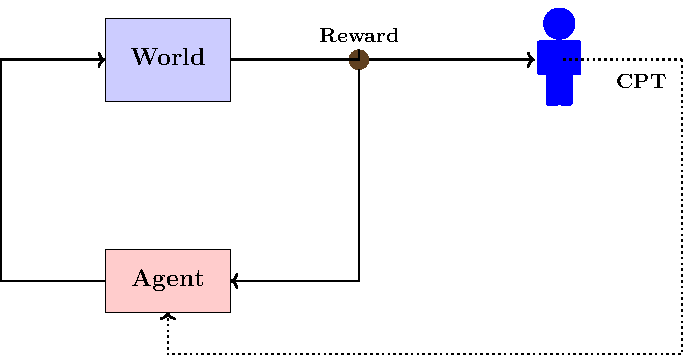
\includegraphics[width=2.3in]{../slides/fig/human-system-figure.pdf}}
\end{center}

\begin{small}

\begin{center}
\tikz[baseline]{
            \node[fill=red!20,anchor=base] (t1)
{\makecell{\textit{\textbf{Cumulative prospect theory (CPT)}} captures\\ \textit{\textbf{human preferences}}}};}
\end{center}
\end{small}
}
%----------------------------------------------------------------------------------------


%----------------------------------------------------------------------------------------
%	SUBCLASSES
%----------------------------------------------------------------------------------------

\headerbox{CPT-value}{name=cptvalue,column=1,row=0,span=2}{
\textbf{\small For a given r.v. $X$, CPT-value $\C(X)$ is}
\begin{align*}
\tikz[baseline]{
            \node[fill=green!20,anchor=base] (t1)
            {$\C(X):= \underbrace{\intinfinity w^+\left(\Prob{u^+(X)>z}\right) dz}_{\textbf{Gains}} - \underbrace{\intinfinity w^-\left(\Prob{u^-(X)>z}\right) dz}_{\textbf{Losses}}$};        }
\end{align*}
\begin{scriptsize}
\textbf{Utility functions} $u^+,u^-:\R\rightarrow \R_+$, $u^+(x)=0$ when $x\le 0$, $u^-(x)=0$ when $x\ge 0$

\textbf{Weight functions} $w^+,w^-:[0,1] \rightarrow [0,1]$ with $w(0)=0$, $w(1)=1$
\end{scriptsize}

\vspace{1ex}

\textbf{\small Connection to expected value:} Letting {$(a)^+ = \max(a,0)$, $(a)^- = \max(-a,0)$}, we have
\begin{align*}
\tikz[baseline]{
            \node[fill=red!20,anchor=base] (t1)
            {\makecell{$\C(X) = \intinfinity \Prob{X>z} dz -  \intinfinity \Prob{-X>z} dz
						= \EE{ (X)^+ } - \EE{ (X)^- }$}};
        }
\end{align*}
}
%----------------------------------------------------------------------------------------

%----------------------------------------------------------------------------------------
%	Tversky-Kahneman
%----------------------------------------------------------------------------------------

\headerbox{Prospect Theory}{name=pt,column=0,below=humansystems}{
\begin{tabular}{cc}
\begin{minipage}{0.45\textwidth}
\includegraphics[height=1.25in]{../slides/fig/tversky.jpg}  

\textbf{~Amos Tversky}
\end{minipage}
&
\begin{minipage}{0.45\textwidth}
\includegraphics[height=1.25in]{../slides/fig/kahneman.jpeg}  

\textbf{~Daniel Kahneman}
\end{minipage}
\end{tabular}

\vspace{1ex}

\begin{scriptsize}
  Kahneman \& Tversky (1979) ``\textit{Prospect Theory: An analysis of decision under risk}'' is the second most cited paper in economics during the period, 1975-2000 
\end{scriptsize}
}
%----------------------------------------------------------------------------------------

%----------------------------------------------------------------------------------------
%	utils
%----------------------------------------------------------------------------------------

\headerbox{Utility functions}{name=utils,column=1,below=cptvalue}{
%\begin{tabular}{cc}
%\begin{minipage}{0.5\textwidth}
%\textbf{\color{bleu1}\small Utility functions}\\[2ex]

   \scalebox{0.7}{\begin{tikzpicture}
   \begin{axis}[width=11cm,height=6.5cm,legend pos=south east,
          %  grid = major,         
            axis lines=middle,
           % grid style={dashed, gray!30},
            xmin=-5,     % start the diagram at this x-coordinate
            xmax=5,    % end   the diagram at this x-coordinate
            ymin=-4,     % start the diagram at this y-coordinate
            ymax=4,   % end   the diagram at this y-coordinate
           % axis background/.style={fill=white},
            ylabel={\large\bf Utility},
            xlabel={\large\bf Gains},
            x label style={at={(axis cs:4.7,-0.8)}},
            y label style={at={(axis cs:-0.8,4.8)}},
            xticklabels=\empty,
            yticklabels=\empty
            ]
           \addplot[name path=cptplus,domain=0:5, green!35!black, very thick,smooth] 
              {pow(abs(x),0.8)}; 
            \addplot[name path=cptminus,domain=-5:0, red!35!black,very thick,smooth] 
              {-2*pow(abs(x),0.7)}; 
               \addplot[domain=-5:5, blue, thick]           {x}; 
               
               \path[name path=diagplus] (axis cs:0,0) -- (axis cs:5,5);
 			  \path[name path=diagminus] (axis cs:-5,-5) -- (axis cs:0,0);
                \path[name path=xaxisplus] (axis cs:0,0) -- (axis cs:5,0);
                 \path[name path=xaxisminus] (axis cs:-5,0) -- (axis cs:0,0);
                 \path[name path=yaxisplus] (axis cs:0,0) -- (axis cs:0,5);
                 \path[name path=yaxisminus] (axis cs:0,-5) -- (axis cs:0,0);
 
 \addplot [orange!40]  fill between[of= diagminus and yaxisminus];
 \addplot [cyan!20]  fill between[of= diagplus and xaxisplus];
 
 \node at (axis cs:  -3.7,-0.45) {\large\bf Losses};
 \node at (axis cs:  4,2.5) {\large $\bm{u^+}$};
 \node at (axis cs:  -1,-3) {\large $\bm{-u^-}$};
 %\node at (axis cs:  2.5,-2.5) {\large\bf Reference point};
%\draw[-{>[scale=2.5,
          %length=5,
          %width=3]},thick] (axis cs:2,-2) -- (axis cs:0,0);
   \end{axis}
   \end{tikzpicture}}

%A reference point on the $x$ axis serves as the point of separating gains and losses.
%For losses, the disutility $-u^-$ is typically convex, for gains, the utility $u^+$ is typically concave; 
%they are always non-decreasing and both of them take on the value of zero at the reference point.
\begin{center}
\begin{small}
\tikz[baseline]{
            \node[fill=red!20,anchor=base] (t1)
{\makecell{For losses, the disutility $-u^-$ is \textbf{convex},\\
 for gains, the utility $u^+$ is \textbf{concave}}};}
\end{small}
\end{center}
%\end{minipage}
}
%----------------------------------------------------------------------------------------

%----------------------------------------------------------------------------------------
%	Weights
%----------------------------------------------------------------------------------------

\headerbox{Weight functions}{name=weights,column=2,below=cptvalue}{
  \centering
  \scalebox{0.7}{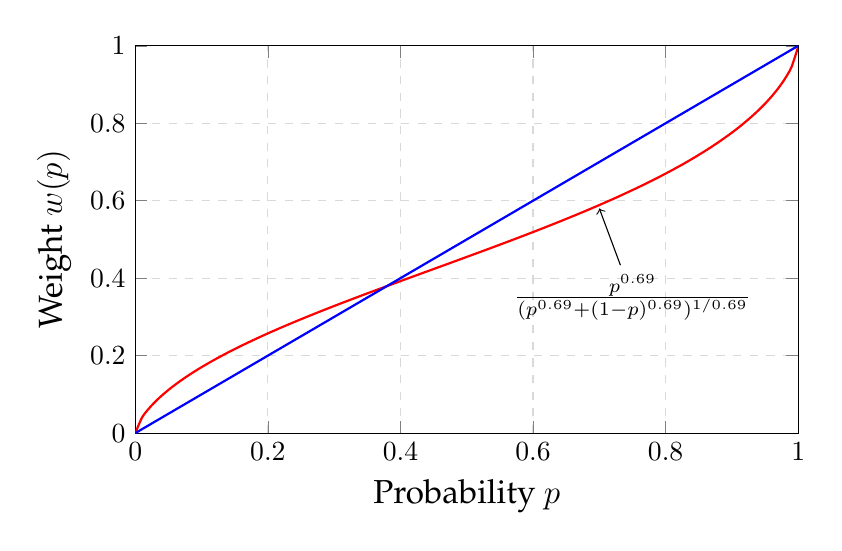
\begin{tikzpicture}
  \begin{axis}[width=10cm,height=6.5cm,legend pos=south east,
           grid = major,
           grid style={dashed, gray!30},
           xmin=0,     % start the diagram at this x-coordinate
           xmax=1,    % end   the diagram at this x-coordinate
           ymin=0,     % start the diagram at this y-coordinate
           ymax=1,   % end   the diagram at this y-coordinate
           axis background/.style={fill=white},
           ylabel={\large Weight $\bm{w(p)}$},
           xlabel={\large Probability $\bm{p}$}
           ]
          \addplot[domain=0:1, red, thick,smooth, samples=100] 
             {pow(x,0.69)/pow((pow(x,0.69) + pow(1-x,0.69)),1.44)}; 
             \node at (axis cs:  0.75,0.35) (a1) {$\bm{\frac{p^{0.69}}{(p^{0.69}+ (1-p)^{0.69})^{1/0.69}}}$};           
             \draw[->] (a1) -- (axis cs:  0.7,0.58);
                 \addplot[domain=0:1, blue, thick]           {x};                      
  \end{axis}
  \end{tikzpicture}}
\begin{small}
\begin{center}
\tikz[baseline]{
            \node[fill=red!20,anchor=base] (t1)
{\makecell{\textbf{Overweight} low probabilities,\\
 \textbf{underweight} high probabilities}};}
\end{center}
\end{small}
}
%----------------------------------------------------------------------------------------

%----------------------------------------------------------------------------------------
%	Prediction
%----------------------------------------------------------------------------------------

\headerbox{CPT-value prediction using empirical distributions}{name=edf,column=0,below=pt, span=2}{
\textbf{\color{red} Problem:} Given samples $X_1, \ldots, X_n$ from the distribution $F(X)$, estimate
%
\tikz[baseline]{
            \node[fill=blue!20,anchor=base] (t1)
            {\makecell{$\C(X):= \intinfinity w^+\left(\Prob{u^+(X)>z}\right) dz - \intinfinity w^-\left(\Prob{u^-(X)>z}\right) dz$}};
        }
\ \\[1.5ex]				
\textbf{Why is it difficult?}:
Samples are from $F(X)$, but $\C(X)$ {\color{red}distorts} 
$\Rightarrow$ Sample means {\color{red} won't} work

\vspace{1ex}

\begin{tabular}{c|c}
\begin{minipage}{0.6\textwidth}
%
\begin{align*}
\tikz[baseline]{
            \node[fill=blue!20,anchor=base] (t1)
            {Let ${\hat F_n}^+(x)=\frac{1}{n} \sum_{i=1}^n 1_{(u^+(X_i) \leq x)}, \quad {\hat F_n}^-(x)=\frac{1}{n} \sum_{i=1}^n 1_{(u^-(X_i) \leq x)}$};
        }
\end{align*}

\vspace{1ex}
%\pause

Using EDFs, the CPT-value $\C(X)$ is estimated by
\begin{align*}
\tikz[baseline]{
            \node[fill=red!20,anchor=base] (t1)
            {
$\overline \C_n = \underbrace{\intinfinity w^+(1-{\hat F_n}^+(x))  dx}_{\textbf{Part (I)}} - \underbrace{\intinfinity w^-(1-{\hat F_n}^-(x))  dx}_{\textbf{Part (II)}}$
};
        }
        \end{align*}


\textbf{Computing Part (I):} Let $X_{[1]}, X_{[2]}, \ldots ,X_{[n]}$ denote the order-statistics 				
        \begin{align*}
\tikz[baseline]{
            \node[fill=green!20,anchor=base] (t1)
            {
$\textbf{Part (I)} = \sum_{i=1}^{n} u^+(X_{[i]}) \left(w^+\!\left(\frac{n+1-i}{n}\right)\!-\! w^+\!\left(\frac{n-i}{n}\right) \right),$
};
        }
        \end{align*}
\end{minipage}
&
\begin{minipage}{0.35\textwidth}
{\textbf{(A1).}  \textbf{\holder continuous} $w^+, w^-$\\ $| w^+(x) - w^+(y) | \leq H | x-y |^{\alpha}, \forall x,y$}\\[2ex]
{\textbf{(A2).}  Utilities $u^+(X)$ and $u^-(X)$ are bounded above by $M<\infty$}

{\color{blue}\textbf{Sample Complexity:}}\\[1ex]
%Under (A1) and (A2), 
For any $\epsilon, \delta >0$, we have
\begin{align*}
\tikz[baseline]{
            \node[fill=pink!20,anchor=base] (t1)
            {
\makecell{$\Prob{\left |\overline \C_n- \C(X) \right| \leq  \epsilon } >1- \delta,$\\[0.5ex]
$ \forall n \geq \ln\left(\frac{1}{\delta}\right)\cdot 
\frac{4H^2 M^2}{\epsilon^{2/\alpha}}$}};}
\end{align*}

\textbf {\color{darkgreen}Case $\alpha=1$ (Lipschitz weights):} \\
%\begin{quote}
\tikz[baseline]{
            \node[fill=red!20,anchor=base] (t1)
            {\makecell{Sample complexity $O\left(1/\epsilon^2\right)$\\ for accuracy $\epsilon$}};
        }
%\end{quote} 
\end{minipage}
\end{tabular}

}
%----------------------------------------------------------------------------------------

%----------------------------------------------------------------------------------------
%	CPT-Val optimization
%----------------------------------------------------------------------------------------

\headerbox{CPT-value optimization using SPSA}{name=cptOptimize,column=0,below=edf,span=2}{
\begin{tabular}{c|c|c}
\begin{minipage}{0.35\textwidth}

\tikz[baseline]{
            \node[fill=magenta!20,anchor=base] (t1)
            {$\textrm{Find ~}\theta^* = \argmax_{\theta \in \Theta} \C(X^\theta)$};
        }
\\				
{\scriptsize \textbf{\color{bleu2} RL:} $\theta = $ policy parameter,  $X^\theta = $ return}
\\[1ex]
	      %\begin{figure}
      \tikzset{
	  %Define standard arrow tip
	  >=stealth',
	  %Define style for boxes
	  punkt/.style={
		rectangle,
		rounded corners,
		draw=black, very thick,
		text width=7.5em,
		minimum height=3.5em,
		text centered},
	  % Define arrow style
	  pil/.style={
		->,
		thick,
		shorten <=2pt,
		shorten >=2pt,}
      }
      %\textbf{Policy iteration principle central to LSPI}
      \centering
      \scalebox{0.45}{\begin{tikzpicture}[node distance=1cm, auto,]
      %nodes
      \node (dummy) {};
      \node[punkt,fill=blue!20,above=1cm of dummy] (peval) {\bf Prediction};
      \node[punkt, fill=red!20,inner sep=5pt,below=1cm of dummy]
      (pimp) {\bf Control};
      % We make a dummy figure to make everything look nice.
      \node[right=2cm of dummy] (t) {\bf CPT-value $\bm{\C^\theta}$}
	edge[pil,<-,bend right=45] (peval.east) % edges are used to connect two nodes
	edge[pil, bend left=45] (pimp.east); % .east since we want
						  % consistent style
      \node[left=2cm of dummy] (g) {\bf Parameter $\bm{\theta}$}
	edge[pil, bend left=45] (peval.west)
	edge[pil,<-, bend right=45] (pimp.west);
      \end{tikzpicture}}

{\bf\color{darkgreen} Two-Stage Solution:}
{\small
\begin{description}
 \item[{\color{darkgreen} Inner stage:}] Obtain $m_n$ samples of $X^{\theta}$ and estimate $\C(X^{\theta})$;
 \vspace{-1.1ex}
 \item[{\color{darkgreen} Outer stage:}] Update $\theta$ using gradient ascent 
 \vspace{-1.1ex}
\end{description}
\textbf{\color{upmaroon}~~$\nabla_{i} \C(X^\theta)$ is not given}}
 \end{minipage}
&
\begin{minipage}{0.35\textwidth}
\begin{small}
\begin{equation*}
\theta^{i}_{n+1} = 
        \tikz[baseline]{
            \node[fill=blue!20,ellipse,anchor=base] (t0)
            {$\Gamma_{i}$};
        } 
\bigg(\theta^{i}_n  +
        \tikz[baseline]{
            \node[fill=blue!20,ellipse,anchor=base] (t1)
            {$\gamma_n$};
        } 
        \tikz[baseline]{
            \node[fill=red!20, anchor=base] (t2)
            {$\widehat \nabla_{i} \C(X^{\theta_n})$};
        }\bigg),%   \quad i=1,\ldots, d.
\end{equation*}

\begin{tabular}[b]{ccc}
\begin{minipage}{0.3\textwidth}
\centering
\tikz[na]\node [coordinate] (n0) {};\textbf{\color{bleu1} Projection operator}           
\end{minipage} 
&
\begin{minipage}{0.25\textwidth}
\centering
\tikz[na]\node [coordinate] (n1) {};          \textbf{\color{bleu2} Step-sizes} 
\end{minipage} 
&
\begin{minipage}{0.25\textwidth}
\centering
\tikz[na]\node [coordinate] (n2) {};  \textbf{\color{vert4}     Gradient estimate} 
\end{minipage}
\end{tabular}

\begin{tikzpicture}[overlay]
        \path[->] (n0) edge [out=145,in=-90] (t0);
        \path[->] (n1) edge [bend left] (t1);
        \path[->] (n2) edge [bend right] (t2);
\end{tikzpicture}

\vspace{1ex}

{\color{red} \textbf{Challenge}:} {estimating $\nabla_{i} \C(X^\theta)$
given only biased estimates of $\C(X^\theta)$}

\vspace{1ex}

{\bf\color{darkgreen} Solution: use SPSA [Spall'92]}
\begin{align*}
\widehat \nabla_{i} \C(X^\theta) = \dfrac{\overline \C_n^{\theta_n+\delta_n \Delta_n} - \overline \C_n^{\theta_n-\delta_n \Delta_n}}{2 \delta_n \Delta_n^{i}}
\end{align*}
{\scriptsize$\Delta_n$ is a vector of independent Rademacher r.v.s and $\delta_n>0$ vanishes asymptotically.}

\end{small}
\end{minipage}
&
\begin{minipage}{0.35\textwidth}
\tikzstyle{block} = [draw, fill=white, rectangle,
   minimum height=5em, minimum width=6em]
\tikzstyle{sum} = [draw, fill=white, circle, node distance=1cm]
\tikzstyle{input} = [coordinate]
\tikzstyle{output} = [coordinate]
\tikzstyle{pinstyle} = [pin edge={to-,thin,black}]

\textbf{\small\color{upmaroon} Simulation optimization}\\[0.5ex]
\scalebox{0.6}{\begin{tikzpicture}[auto, node distance=2cm,>=latex']
% We start by placing the blocks
\node (theta) {$\boldsymbol{x}$};
\node [block, fill=blue!20,right=0.6cm of theta,align=center] (sample) {\makecell{\textbf{Measurement}\\\textbf{ Oracle}}}; 
\node [right=0.6cm of sample] (end) {$\boldsymbol{\mathbf{f(x) + \xi}}$};
\node [ below= 0.6cm of end] (bias) {\textbf{Zero mean}};
\draw [->] (theta) --  (sample);
\draw [->] (sample) -- (end);
\path [darkgreen,->] (bias) edge [bend right] (end.east);
\end{tikzpicture}}


\vspace{1ex}

\textbf{\small \color{shockingpink} CPT-value optimization}\\[0.5ex]
\scalebox{0.6}{\begin{tikzpicture}[auto, node distance=2cm,>=latex']
% We start by placing the blocks
\node (theta) {$\boldsymbol{X, \epsilon}$};
\node [block, fill=blue!20,right=0.6cm of theta,align=center] (sample) {\makecell{\textbf{CPT}\\\textbf{ Estimator}}}; 
\node [right=0.6cm of sample] (end) {$\boldsymbol{\mathbf{\C(X) + \epsilon}}$};
\node [ below= 0.6cm of end] (bias) {\makecell{\textbf{Controlled}\\ \textbf{bias}}};
\draw [->] (theta) --  (sample);
\draw [->] (sample) -- (end);
\path [red,->] (bias) edge [bend right] (end.east);
\end{tikzpicture}}

\vspace{1ex}

{\small How to choose $m_n$ to \\ignore estimation bias?\\[1ex]
\tikz[baseline]{
            \node[fill=red!20,anchor=base] (t1)
            {\makecell{Ensure $\frac{1}{m_n^{\alpha/2}\delta_n}\rightarrow 0$}};}
        }


\end{minipage}

\end{tabular}


}
----------------------------------------------------------------------------------------

%----------------------------------------------------------------------------------------
%	Experiments
%----------------------------------------------------------------------------------------

\headerbox{Traffic delay optimization}{name=traffic,column=2, below=weights,span=1}{
\begin{tabular}[b]{c}
\begin{minipage}{\textwidth}
\centering
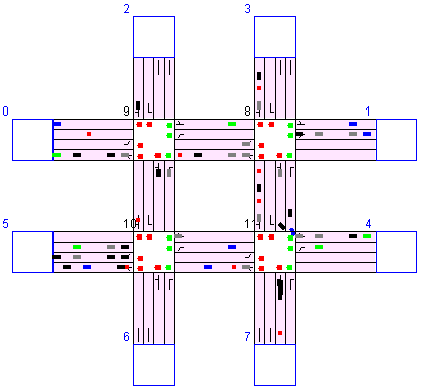
\includegraphics[width=2in, height=1.1in]{../slides/fig/2x2grid.png}
\end{minipage} \\
\begin{minipage}{\textwidth}

\vspace{1ex}

{\small Maximize \tikz[baseline]{
            \node[fill=red!20, anchor=base] (t2)
            {$\text{CPT}(X_1,\ldots,X_{\M}) = \sum_{i=1}^{\M} \mu^i \C(X_i)$,};
        }\\
$X_i =$ delay gain for path $i=1,\ldots,\M$}\\[1ex]
\textbf{AVG-SPSA (uses plain sample means)}\\[1ex]
\tabl{c}{\scalebox{0.5}{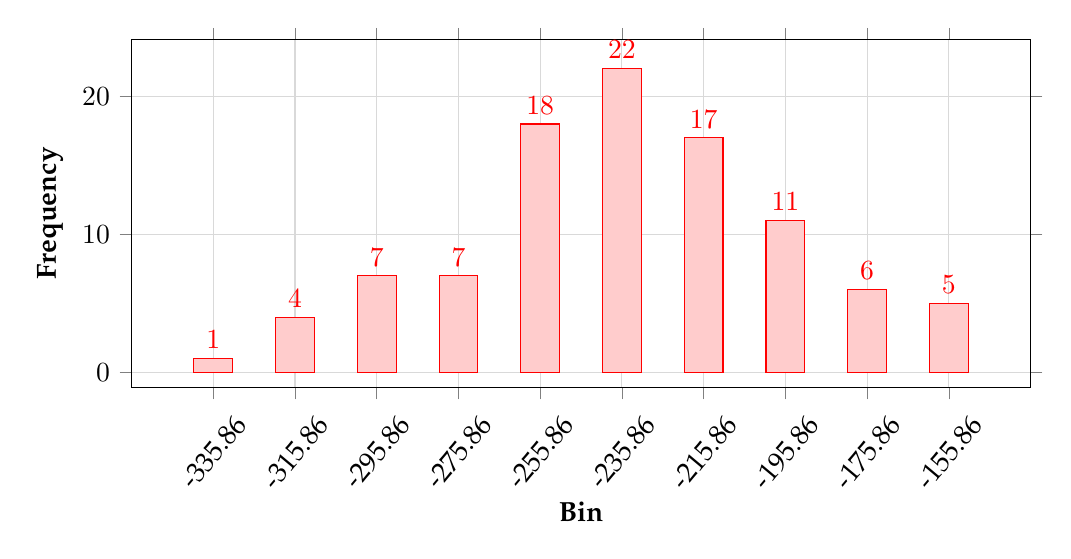
\begin{tikzpicture}
\begin{axis}[
ybar={2pt},
%  legend style={at={(0.5,-0.2)},anchor=north,legend columns=-1},
legend pos=outer north east,
legend image code/.code={\path[fill=white,white] (-2mm,-2mm) rectangle
(-3mm,2mm); \path[fill=white,white] (-2mm,-2mm) rectangle (2mm,-3mm); \draw
(-2mm,-2mm) rectangle (2mm,2mm);},
ylabel={\bf Frequency},
xlabel={\textbf{Bin}},
x label style={at={(axis description cs:0.5,-0.3)},anchor=north},
symbolic x coords={0, -335.86, -315.86, -295.86, -275.86, -255.86, -235.86, -215.86, -195.86, -175.86, -155.86, 11},
xmin={0},
xmax={11},
xtick=data,
ytick align=outside,
%xticklabels={{\bf7x9-Grid\\[0.5ex]($d=504$),\bf 14x9-Grid\\[0.5ex]($d=1008$),\bf 14x18-Grid\\[0.5ex]($d=2016$),\bf 28x18-Grid\\[0.5ex]($d=4032$)}},
xticklabel style={rotate=50, align=center},
bar width=14pt,
nodes near coords,
grid,
grid style={gray!30},
width=13cm,
height=6cm,
]
\addplot[red, fill=red!20]   coordinates {  (-335.86,1) (-315.86,4) (-295.86,7) (-275.86,7) (-255.86,18) (-235.86,22) (-215.86,17) (-195.86,11) (-175.86,6) (-155.86,5)}; %LSPI
\end{axis}
\end{tikzpicture}}}
\end{minipage} \\
\begin{minipage}{\textwidth}
\textbf{EUT-SPSA (uses utilities but no weights)} \\[1ex]
\tabl{c}{\scalebox{0.5}{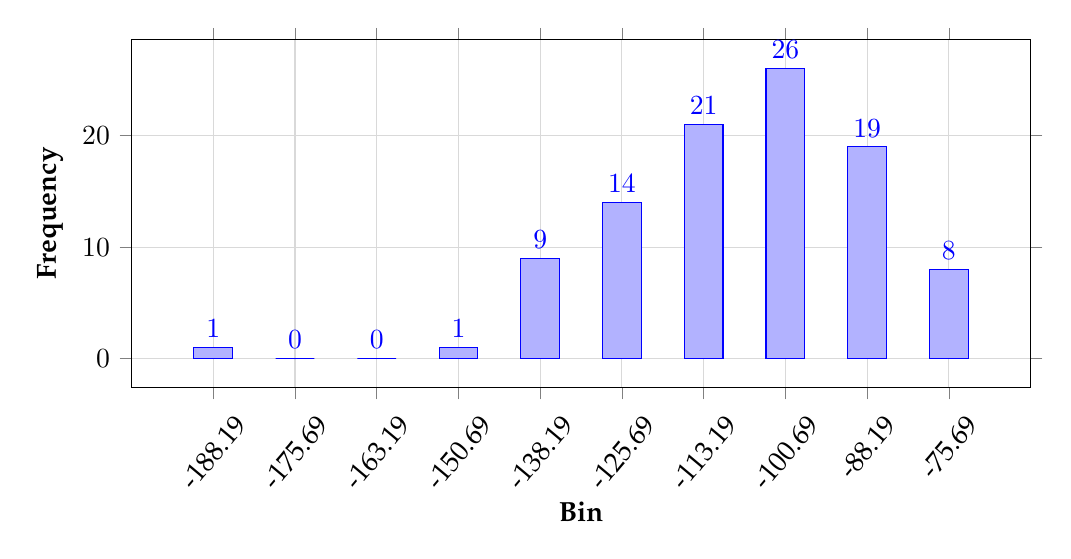
\begin{tikzpicture}
\begin{axis}[
ybar={2pt},
%  legend style={at={(0.5,-0.2)},anchor=north,legend columns=-1},
legend pos=outer north east,
legend image code/.code={\path[fill=white,white] (-2mm,-2mm) rectangle
(-3mm,2mm); \path[fill=white,white] (-2mm,-2mm) rectangle (2mm,-3mm); \draw
(-2mm,-2mm) rectangle (2mm,2mm);},
ylabel={\bf Frequency},
xlabel={\textbf{Bin}},
x label style={at={(axis description cs:0.5,-0.3)},anchor=north},
symbolic x coords={0,-188.19,-175.69,-163.19,-150.69,-138.19,-125.69,-113.19,-100.69,-88.19,-75.69,11},
xmin={0},
xmax={11},
xtick=data,
ytick align=outside,
%xticklabels={{\bf7x9-Grid\\[0.5ex]($d=504$),\bf 14x9-Grid\\[0.5ex]($d=1008$),\bf 14x18-Grid\\[0.5ex]($d=2016$),\bf 28x18-Grid\\[0.5ex]($d=4032$)}},
xticklabel style={rotate=50, align=center},
bar width=14pt,
nodes near coords,
grid,
grid style={gray!30},
width=13cm,
height=6cm,
]
\addplot   coordinates {  (-188.19,1) (-175.69,0) (-163.19,0) (-150.69,1) (-138.19,9) (-125.69,14) (-113.19,21) (-100.69,26) (-88.19,19) (-75.69,8) }; %LSPI
\end{axis}
\end{tikzpicture}}\\[1ex]}
\end{minipage} \\
\begin{minipage}{\textwidth}
\textbf{CPT-SPSA (uses both utilities and weights)} \\[1ex]
\tabl{c}{\scalebox{0.5}{\begin{tikzpicture}
\begin{axis}[
ybar={2pt},
%  legend style={at={(0.5,-0.2)},anchor=north,legend columns=-1},
legend pos=outer north east,
legend image code/.code={\path[fill=white,white] (-2mm,-2mm) rectangle
(-3mm,2mm); \path[fill=white,white] (-2mm,-2mm) rectangle (2mm,-3mm); \draw
(-2mm,-2mm) rectangle (2mm,2mm);},
ylabel={\bf Frequency},
xlabel={\textbf{Bin}},
x label style={at={(axis description cs:0.5,-0.25)},anchor=north},
symbolic x coords={0, -43.36,-33.36,-23.36,-13.36,-3.36,6.64,16.64,26.64,36.64,46.64, 11},
xmin={0},
xmax={11},
xtick=data,
ytick align=outside,
%xticklabels={{\bf7x9-Grid\\[0.5ex]($d=504$),\bf 14x9-Grid\\[0.5ex]($d=1008$),\bf 14x18-Grid\\[0.5ex]($d=2016$),\bf 28x18-Grid\\[0.5ex]($d=4032$)}},
xticklabel style={rotate=50, align=center},
bar width=14pt,
nodes near coords,
grid,
grid style={gray!30},
width=13cm,
height=6cm,
]
\addplot[darkgreen, fill=darkgreen!20]   coordinates {  (-43.36,1) (-33.36,0) (-23.36,0) (-13.36,1) (-3.36,0) (6.64,1) (16.64,8) (26.64,52) (36.64,24) (46.64,12) }; %LSPI
\end{axis}
\end{tikzpicture}}}
\end{minipage} 
\end{tabular}
}
%----------------------------------------------------------------------------------------


\end{poster}

\end{document}